\documentclass[main_estudante.tex]{subfiles}

\begin{document}

\chapter{Equação de retas e circunferências}

\section{Apresentação}

Parte da disciplina Geometria Analítica se dedica a estudar as expressões algébricas que representam curvas importantes por sua simplicidade, generalidade ou aplicações específicas. Dentre essas curvas podemos mencionar retas, planos, circunferências, cônicas e quádricas. Neste capítulo, vamos estudar retas e circunferências no plano visando explorar aspectos que serão úteis no estudo das demais curvas mencionadas tanto no plano quanto no espaço.

\section{Pré-requisitos e Auto-avaliação inicial}

Os pré-requisitos para este capítulo são:
\begin{itemize}
 \item Equação da reta;
 \item Distância entre pontos no plano.
\end{itemize}

Esses tópicos não serão cobertos durante as atividades de tutoria. Se você acha que não sabe o suficiente sobre algum deles, sugerimos que se procure material de apoio antes de começar a resolver as questões desse capítulo.

Antes de começar, indique o quanto você acha que sabe sobre os seguintes itens:

\begin{center}
 \begin{tabular}{|p{35mm}||p{15mm}|p{15mm}|p{15mm}|p{15mm}|} 
 \hline
   & Nada & Muito pouco & Noções gerais & Bastante\\
 \hline
 Traçar o gráfico de uma reta dada a sua equação &  &  &  &  \\ 
 \hline
 Obter a equação de uma reta dados dois pontos &  &  &  &  \\
 \hline
 Identificar a equação de uma circunferência &  &  &  &  \\
 \hline
\end{tabular}
\end{center}

\newpage

\section{Questões diagnósticas}

\begin{diagnostico}
Considere os pontos $P=(1;3)$ e $Q=(-1;-1)$.
\begin{enumerate}[a)]
\item Obtenha a equação da reta que passa pelos dois pontos.
\item Dê a equação de uma reta diferente e paralela à encontrada no item a.
\end{enumerate}
\end{diagnostico}

\vspace{4cm}

\begin{diagnostico}
Considere as retas dadas pelas equações $2y+3x-1=0$ e $y-4x+3=0$.
\begin{enumerate}[a)]
\item Obtenha o ponto de intersecção entre as duas retas.
\item Represente as retas em um plano cartesiano.
\end{enumerate}
\end{diagnostico}

\newpage

\section{Questões}

Vamos começar esse capítulo com uma das propriedades básicas das retas no plano: dois pontos determinam uma reta.

\subsection*{Pontos e retas}

\begin{questao}
Considere os pontos $P=(1;1)$ e $Q=(3;5)$.
\begin{enumerate}[a)]
\item Marque os dois pontos em um eixo cartesiano.
\item Trace a reta que passa pelos dois pontos.
\item Avaliando visualmente, você diria que quais dos seguintes pontos estão sobre a reta: $A=(-1;2)$,$B=(4;4)$, $C=(2;3)$, $D=(-1;-3)$?
\item Avaliando visualmente, em quais pontos essa reta parece cortar os eixos $X$ e $Y$?
\end{enumerate}
\end{questao}

Para traçar a reta na questão acima, você provavelmente posicionou a sua régua sobre os dois pontos que havia marcado no eixo cartesiano. Ao posicionar sobre os dois pontos a régua ficou com a sua posição totalmente definida (um ponto só permitiria girar a régua). Esse é o significado concreto da propriedade ``dois pontos determinam uma única reta''.

\subsection*{Equação da reta}

O equivalente algébrico da propriedade mencionada acima é que dados dois pontos (diferentes) temos informação suficiente para determinar a equação da reta que passa por eles. 

Existem vários métodos para resolver essa questão, mas se você não sabe como obter a equação de uma reta a partir de dois pontos, peça ajuda a um colega ou ao tutor para resolver a questão a seguir.

\begin{questao}
Obtenha a equação da reta que passa pelos pontos $P=(1;1)$ e $Q=(3;5)$.
\end{questao}

Você deve ter obtido a equação $y=2x-1$ na questão acima, entretanto, essa reta poderia ser representada algebricamente por expressões que, apesar de serem equivalentes a essa, tem um formato bastante diferente. Esses diferentes formatos e suas propriedades é um dos tópicos centrais deste capítulo.

Agora, vamos usar a equação da reta para responder a questões muito parecida com as que foram respondidas visualmente no questão 1.

\begin{questao}
Considere a reta dada pela equação $y=2x-1$, responda:
\begin{enumerate}[a)]
\item Qual é o ponto de coordenada $X$ igual a $10$ que pertence a essa reta?E de coordenada $Y$ igual a $-3$?
\item Em que pontos ela corta os eixos $X$ e $Y$?
\item Quais dos pontos $A=(-1;2)$, $B=(4;4)$, $C=(2;3)$ e $D=(-1;-3)$ pertencem a ela? 
\item Dê as coordenadas de um ponto do quarto quadrante (valores de $X$ positivos e de $Y$ negativos) que pertença à reta.
\end{enumerate} 
\end{questao}

\subsection*{Equação da reta na forma reduzida}

Chamamos de \textbf{forma reduzida} a equação da reta dada no formato $y=mx+c$. Esse formato é bastante comum pois é conveniente também para o estudo de funções (basta usar $f(x)$ ao invés de $y$). Mas além disso, ele possui algumas vantagens.

O valor de $c$ está relacionado com o ponto em que a reta corta o eixo $Y$ e é chamado de \textbf{coeficiente linear}. O valor de $m$, chamado de \texbf{coeficiente angular}, está relacionado com a inclinação da reta: $m>0$ implica uma reta crescente, $m=0$ uma reta horizontal e $m<0$ uma reta decrescente. No geral, essas duas informações são suficientes para um bom esboço da reta em um plano cartesiano.

Se você não sabe como fazer o esboço de uma reta a partir dessas duas informações sem precisar montar uma tabela com pontos, sugerimos uma leitura da seção 3.4 do livro \sugestao{Matemática Básica volume 1} até o final do exemplo 2 antes de resolver a questão abaixo.

\begin{questao}
Usando um único plano cartesiano, esboce as retas dadas pelas equações: $y=x+1$, $y=-2x-4$, $y=\frac{x}{2}$ e $y=\frac{x}{2}-1$.
\end{questao}

Você deve ter notado que duas das retas anteriores são paralelas entre si. Observe as semelhanças e diferenças entre as equações delas e, com base nisso, responda a questão a seguir.

\begin{questao}
Dê a equação de uma reta paralela à reta $y=2x-1$.
\end{questao}

Como você deve ter notado, para que duas retas, dadas na forma reduzida, sejam paralelas basta que seus coeficientes angulares sejam iguais e coeficientes lineares sejam diferentes.

\subsection*{Equação da reta na forma geral}

Um outro formato para a apresentação da equação de uma reta é a chamada \textbf{forma geral}, mostrada abaixo

$$ay+bx+c=0$$

\begin{questao}
Dada a reta de equação $4y+6x-4=0$, faça o que se pede:
\begin{enumerate}[a)]
\item Determine os pontos em que ela corta os eixos $X$ e $Y$.
\item Esboce a reta em um plano cartesino.
\end{enumerate} 
\end{questao}

Note que nesse caso nem a inclinação da reta nem o ponto de intersecção com o eixo $Y$ estão claros na equação da reta. Nesse sentido, a forma geral é menos prática do que a forma reduzida. Porém, ela tem sim algumas vantagens.

\subsection*{Vantagens da forma geral, 1}

A primera delas se refere a possibilidade de representar retas verticais. Por exemplo, a reta vertical que corta o eixo $X$ em $(3;0)$ tem equação $x=3$. Pare e pense. Essa equação pode ser interpretada da seguinte maneira: para qualquer valor de $y$ que você escolher, o valor de $x$ será sempre igual a $3$. Qualquer ponto com $x\neq3$ não pertencerá a essa reta. Isso significa que os pontos dessa reta são exatamente todos os pontos ``empilhados'' verticalmente sobre a marcação $3$ no eixo $x$, ou seja, sobre o ponto $(3;0)$.

Uma reta horizontal que corte o eixo $Y$ no ponto $(0;4)$ terá equação $y=4$. (Pare e pense sobre a interpretação dessa equação).

A diferença entre esses dois casos é que $y=4$ está na forma reduzida (podemos vê-la como $y=0x+4$), mas $x=3$ não (pois precisaríamos de um $0$ multiplicando $y$, o que não pode ocorrer na forma reduzida, pois não há uma constante multiplicando $y$). Entretanto, ambas as equações e encaixam na forma geral: $x-3=0$ (que pode ser vista como $0y+x-3=0$) e $y-4=0$ (que pode ser vista como $y+0x-4=0$).

Portanto, a forma geral comporta casos válidos do ponto de vista geométrico que a forma reduzida não comporta.

\begin{questao}
Esboce o gráfico das retas com equações iguais a $x-5=0$, $y+1=0$, $2x+1=0$ e $y=0$.
\end{questao}

\subsection*{Vantagens da forma geral, 2}

Outra vantagem da forma geral se refere ao \textbf{vetor normal} à reta. Esse é o nome dado a um vetor (qualquer um deles) que seja perpendicular à reta. Esse vetor é muito importante para obtermos a equação de planos em Geometria Analítica. Para compreendermos essa propriedade, vamos considerar a reta de equação $2y-x-4=0$, que está traçada abaixo.

\begin{figure}[h]
\centering
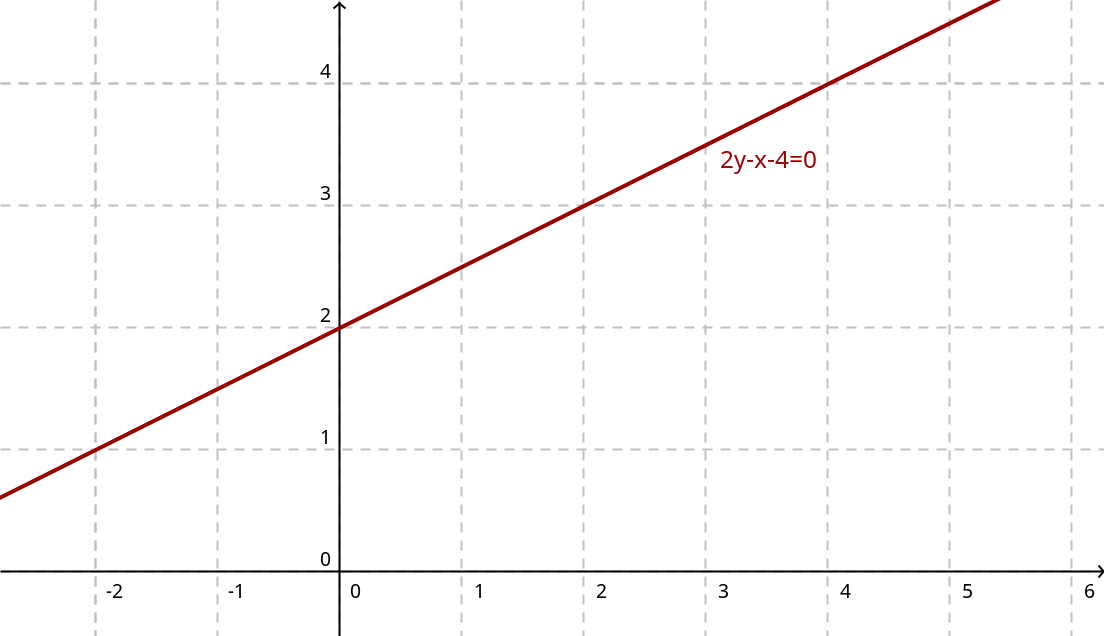
\includegraphics[width=0.7\textwidth]{./img/c6q8.png}
\end{figure}

\begin{questao}
Em relação à reta acima:
\begin{enumerate}[a)]
\item Use o quadriculado para traçar um vetor perpendicular à reta a partir do ponto $(0;2)$. Sugestão: trace um vetor que termine em um dos vértices do quadriculado.
\item Qual é esse vetor?
\end{enumerate} 
\end{questao}

Você deve ter obtido o vetor $\binom{-1}{2}$. Note que as coordenadas $x$ e $y$ desse vetor são iguais aos coeficientes que multiplicam $x$ e $y$ na equação dada. Essa propriedade é bastante poderosa quando lidarmos com planos pois é mais simples indicar a \textbf{direção} de um plano por um vetor normal do que por inclinações em relação aos eixos.

Porém, note também que o vetor normal indica apenas a direção da reta. Ainda nos resta determinar a posição dessa reta. Isso é feito, de maneira geral, dando um ponto que pertence à reta. Dado o vetor normal e mais um ponto, a equação da reta pode ser determinada. 

\begin{questao}
Seja $\overrightarrow{V}=\binom{1}{2}$ e $P=(1;1)$.
\begin{enumerate}[a)]
\item Marque o ponto $P$ no quadriculado abaixo e o vetor $\overrightarrow{V}$ começando em $P$.

\begin{figure}[h]
\centering
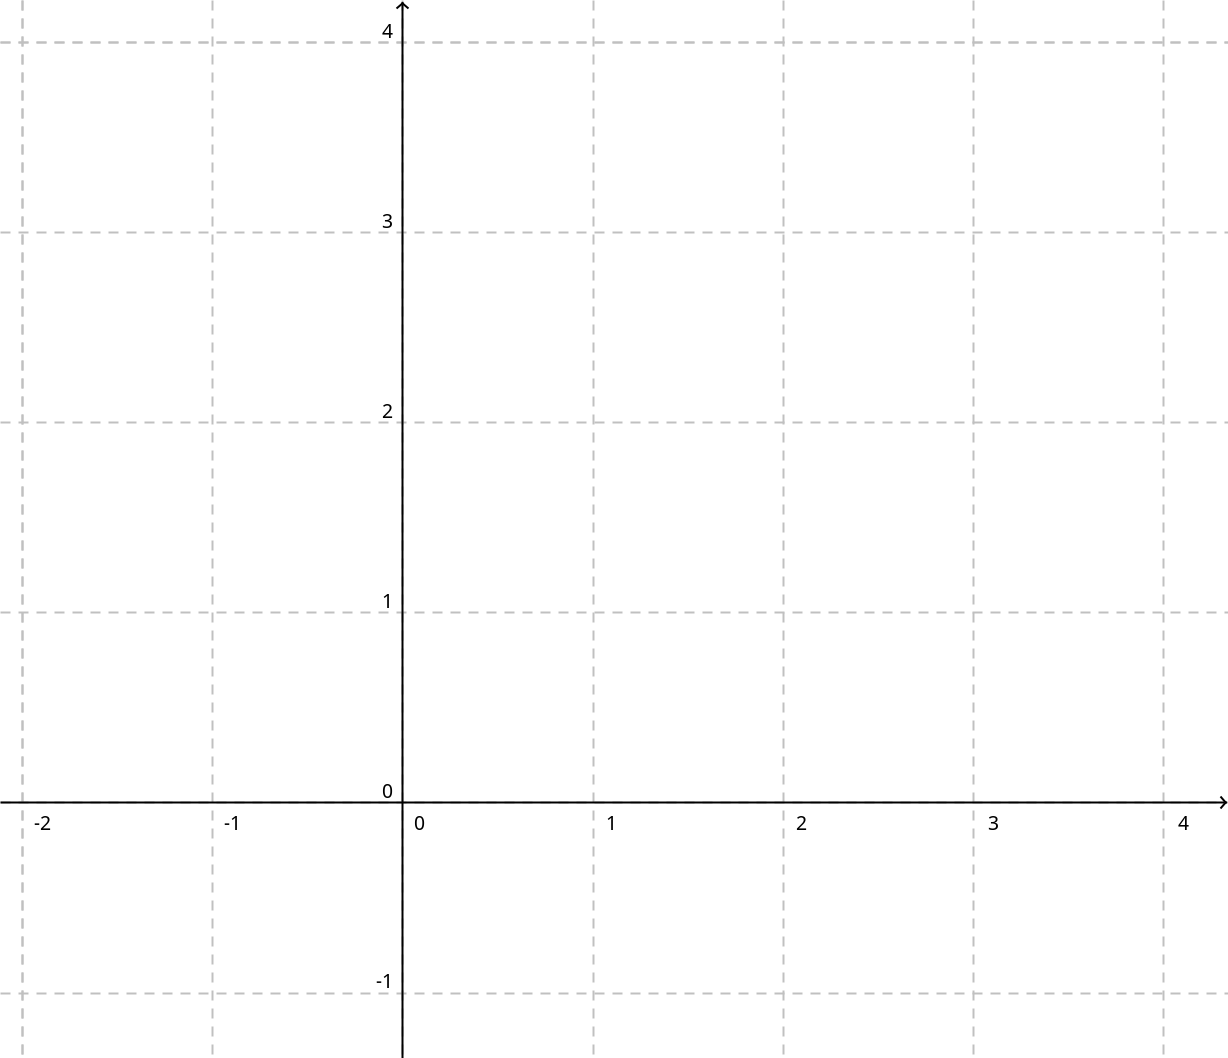
\includegraphics[width=0.7\textwidth]{./img/c6q9.png}
\end{figure}

\item Visualmente, trace uma reta que passa por $P$ e é perpendicular a $\overrightarrow{V}$.
\item Obtenha a equação dessa reta.
\item Obtenha a equação de uma nova reta que passa pelo ponto $Q=(3;2)$ e tem vetor normal igual a $\overrightarrow{U}=\binom{5}{-1}$.
\end{enumerate}
\end{questao}

\begin{reflita}
 Compare com seus colegas o método que você utilizou pra resolver o último item da questão acima e descreva com suas palavras o método que lhe parece o melhor para resolvê-la quando a informação dada é um ponto e o vetor normal da reta.
\end{reflita}


\subsection*{Uma nova forma}

Uma terceira forma de representar algebricamente uma reta é a \textbf{forma paramétrica}. Apesar de ser pouco usada para retas e planos, a forma paramétrica pode facilitar enormemente o tratamento algébrico de algumas curvas e reforça conceitos que serão estudados em Álgebra Linear, como o de combinação linear. Por esse motivo, veremos como utilizá-la.

A ideia por trás de representações paramétricas é a introdução de uma nova variável (parâmetro) que vai ser usada para gerar as coordenadas $X$ e $Y$ de cada ponto pertencente à curva em questão. Isso significa que a expressão não vai relacionar uma coordenada à outra através de uma equação, mas sim usar um parâmetro para gerar os pares de valores para as coordenadas.

Tipicamente, uma equação paramétrica tem o seguinte formato: $(x,y)=(2t-1;4-t^2)$ ou $\begin{cases} x=2t-1 \\ y=4-t^2 \end{cases}$, ambos representando exatamente a mesma curva (que não é uma reta, nesse caso).

Sendo assim, para cada valor de $t$, obtemos valores para as coordenadas $X$ e $Y$ de um ponto que pertence à curva. Por exemplo, para $t=0$ temos o ponto $(-1;4)$ e para $t=1$ temos o ponto $(1;3)$.

Para que uma equação paramétrica no plano seja uma reta, é necessário e suficiente que suas equações sejam lineares em termos de $t$, ou seja, tenham o formato $at+b$. Por exemplo, $(x,y)=(2t-1;t+3)$.

\begin{questao}
Em relação à reta dada pela equação $(x,y)=(2t-1;t+3)$, faça o que se pede.
\begin{enumerate}[a)]
\item Obtenha as coordenadas dos pontos para $t=0$, $t=2$ e $t=-1$.
\item Marque esses pontos no plano cartesiano abaixo e confirme que eles pertencem a uma mesma reta, ou seja, estão alinhados.

\begin{figure}[h]
\centering
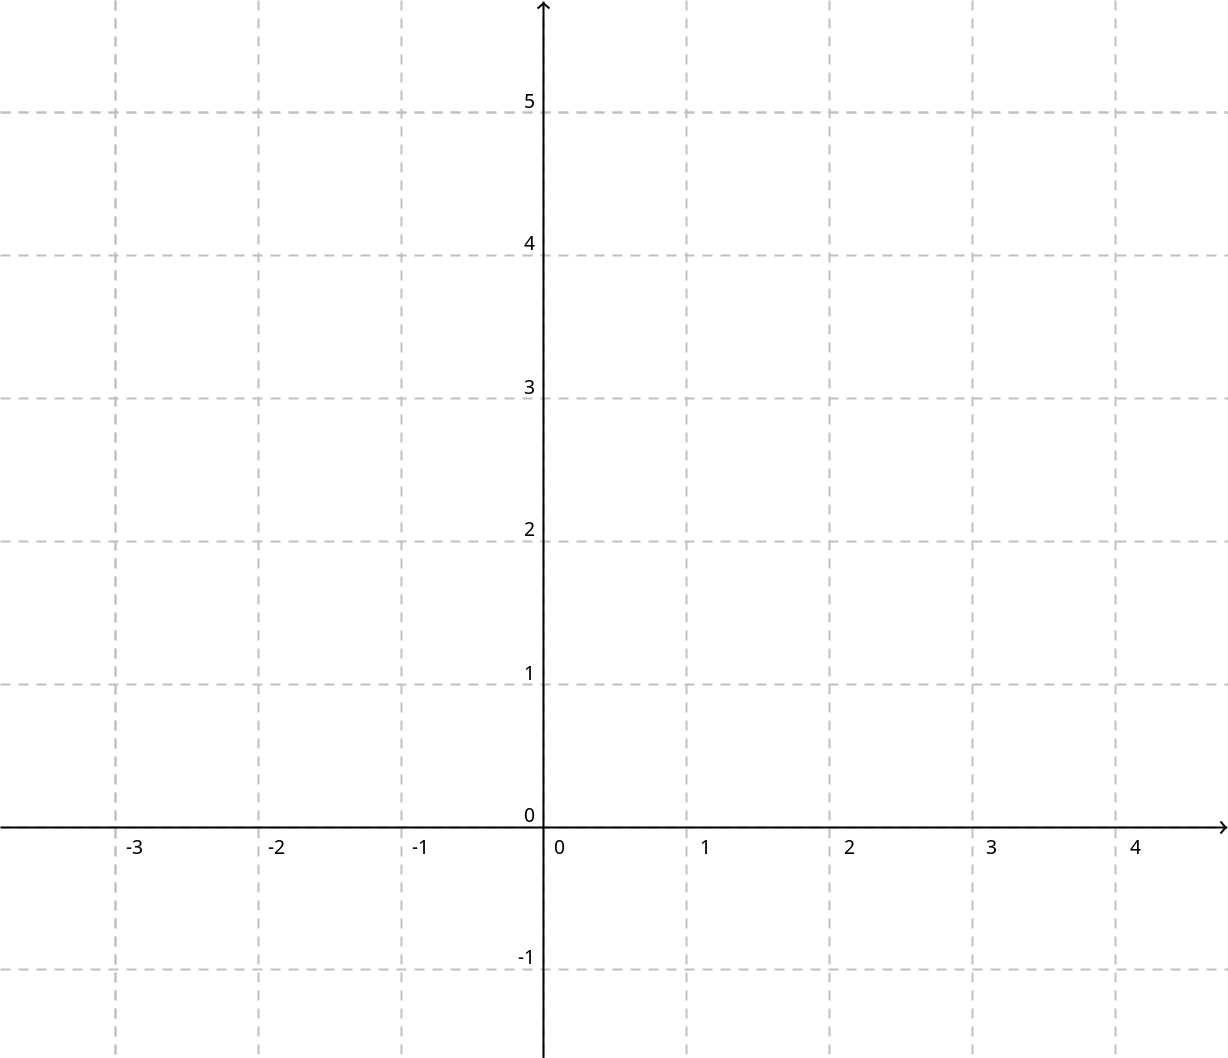
\includegraphics[width=0.7\textwidth]{./img/c6q10.png}
\end{figure}

\item Determine para quais valores de $t$ essa reta cruza os eixos $X$ e $Y$.
\end{enumerate} 
\end{questao}

Essa mesma equação pode ser rescrita como mostrado abaixo.

$$(x,y)=(2t-1;t+3)=(-1+2t;3+t)=(-1;3)+(2t;-t)=(-1;3)+(2;-1) \cdot t$$

A forma mais à direita salienta dois aspectos: o ponto $(-1;3)$ obtido quando $t=0$ que pode ser interpretado como início da curva, e a direção $(2;-1)$ na qual a reta avança à medida que o valor de $t$ aumenta. Dessa maneira, interpretar o parâmetro $t$ como sendo o tempo é um recurso comum neste contexto.

\subsection*{Todas as formas}

\begin{questao}
Considere os pontos $P=(1;1)$ e $Q=(3;5)$.
\begin{enumerate}[a)]
\item Marque esses pontos em um plano cartesiano e trace a reta que passa por eles.
\item Obtenha a equação dessa reta na forma reduzida (suportamente a mais simples para o caso em que dois pontos são dados).
\item Obtenha a equação na forma geral manipulando algebricamente a equação obtida no item anterior.
\item Use a equação na forma geral para obter o vetor normal e trace-o no mesmo plano cartesiano.
\item Obtenha uma equação paramétrca que represente essa mesma reta usando as ideias de ponto inicial e direção da reta.
\end{enumerate} 
\end{questao}

Para finalizar as questões sobre retas, discuta a questão a seguinte usando as respostas obtidas por seus colegas.

\begin{reflita}
Compare com seus colegas para ver se todos obtiveram as mesmas respostas para os itens b, c e e. Em quais desses itens é possível obter respostas diferentes corretas? 
\end{reflita}

\subsection*{Circunferência}

Agora vamos deixar para trás as retas e focar a atenção nas expressões algébricas que representam circunferências.

A forma mais comum de representá-las é a chamada \textbf{forma reduzida}: $(x-x_c)^2+(y-y_c)^2=r^2$, em que $x$ e $y$ são as coordenadas dos pontos que pertencem à circunferência, $x_c$ e $y_c$ são as coordenadas do centro e $r$ é a medida do raio.

Essa expressão é obtida diretamente da definição de circunferência como sendo os pontos $(x;y)$ que estão a uma mesma distante $r$ de um ponto $(x_c;y_c)$ chamado centro. A aplicação do teorema de pitágoras na imagem ao lado gera exatamente a expressão dada acima.

\begin{figure}[h]
\centering
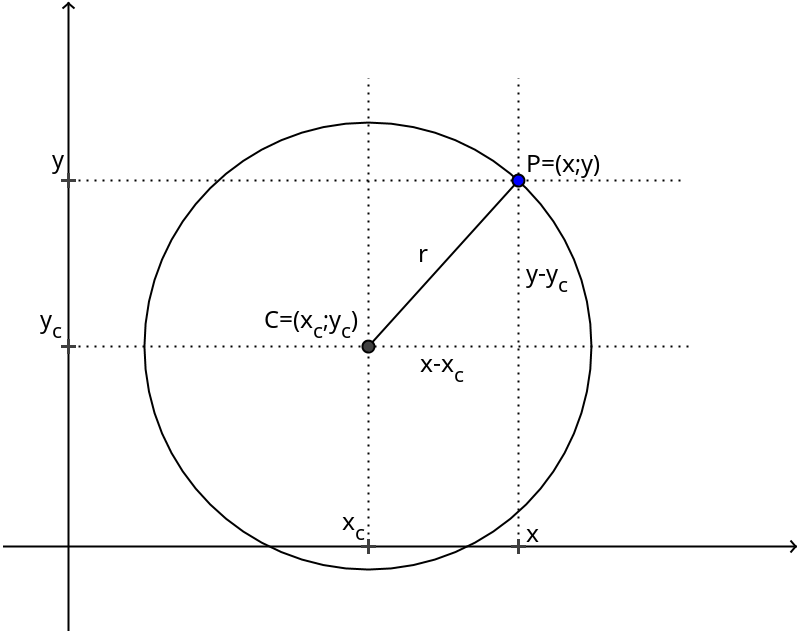
\includegraphics[width=0.5\textwidth]{./img/c6q12.png}
\end{figure}

\begin{questao}
Use a equação dada acima para responder as questões abaixo.
\begin{enumerate}[a)]
\item Qual é a equação da circunferência com centro em $(2;1)$ e raio 3? 
\item Qual é a equação da circunferência com centro na origem e raio 1?
\item Qual é o centro e raio da circunferência dada pela equação $(x-1)^2+(y+3)^2=4$?
\end{enumerate} 
\end{questao}

\subsection*{A forma geral de uma circunferência}

A forma geral de uma circunferência é obtida ao desenvolvermos os quadrados da forma reduzida e simplificarmos a expressão de modo que seja igual a zero. Veja o que ocorre com a equação dada no item c acima.

\begin{align*}
 (x-1)^2+(y+3)^2 &=4 && \text{desenvolvendo as potências}\\
 (x^2-2x+1)+(y^2+6y+9)&=4 && \text{agrupando termos}\\
 x^2-2x+y^2+6y+1+9-4 &=0 && \text{subtraindo 4 dos dois lados}\\
 x^2-2x+y^2+6y+6&=0
 \end{align*}

A última linha acima nos dá a forma geral da equação da circunferência discutida no item c da questão anterior. Note que as coordenadas do centro e o raio da circunferência não são mais claros na expressão. Mesmo assim, essa forma é usada por ser um caso específico de uma família de curvas chamadas cônicas, as quais podem ser descritas por equações com formato muito parecido com a forma geral de uma circunferência. Você estudará essas curvas em breve em Geometria Analítica.

Uma das situações comuns neste contexto é ter que identificar exatamente qual curva é representada por uma equação dada na forma geral. No momento, só conhecemos a circunferência, mas ainda resta o desafio de identificar seu centro e raio dada a sua equação na forma geral.

Vejamos o que poderia ser feito em relação à equação $x^2+8x+y^2-6y-11=0$. Primeiro, note que o termo independente, $-11$ é bem pouco útil, pois ele é o resultado da soma do termo independente resultante do primeiro quadrado, do segundo quadrado e do quadrado do raio. Os termos $x^2$ e $y^2$ também não oferecem muita informação sobre a forma reduzida, mas os termos $8x$ e $-6y$ podem ser úteis. Ambos são resultados puros de expressões do tipo $(x+a)^2$ e $(y+b)^2$. Tendo em mente que $(x+a)^2=x^2+2ax+a^2$, descobrimos que $8x$ só pode ter vindo de um expressão do tipo $(x+4)^2$ e $-6y$ de $(y-3)^2$. Logo, a forma reduzida da nossa circunferência deve ser $(x+4)^2+(y-3)^2=r^2$, ou seja, já sabemos que o centro da circunferência é $(-4;3)$.

Agora, vamos focar no raio. Se desenvolvermos os quadrados da expressão acima, obtemos $x^2+8x+y^2-6y+25-r^2=0$. Logo, $25-r^2=-11$, o que implica que $r=6$. Portanto, a circunferência de equação $x^2+8x+y^2-6y-11=0$ tem centro em $(-4;3)$ e raio igual a $6$.

\begin{questao}
Obtenha o raio e centro da circunferência dada pela equação $x^2+2x+y^2-8y+13=0$
\end{questao}

Como esse tipo de questão será comum logo mais em Geometria Analítica propomos mais uma questão similar para ser resolvida com um colega.

\begin{questao}
Visando praticar um pouco mais o uso da forma geral de uma circunferência, faça o que se pede a seguir:
\begin{enumerate}[a)]
\item Escolha o centro e raio de uma circunferência, escreva a sua forma reduzida e desenvolva-a de modo a obter a sua forma geral.
\item Passe apenas a forma geral para um colega e obtenha o centro e raio da circunferência por trás da forma geral que ele te passou.
\item Cheque se ambos acertaram a questão.
\end{enumerate} 
\end{questao}
 
\subsection*{A forma paramétrica de uma circunferência}

A equação paramétrica da circunferência é especialmente importante por oferecer uma conexão entre expressões do tipo polinomial e as relações trigonométricas. Vamos focar nas circunferências de raio $1$ com centro na origem, como mostrado abaixo.

\begin{figure}[h]
\centering
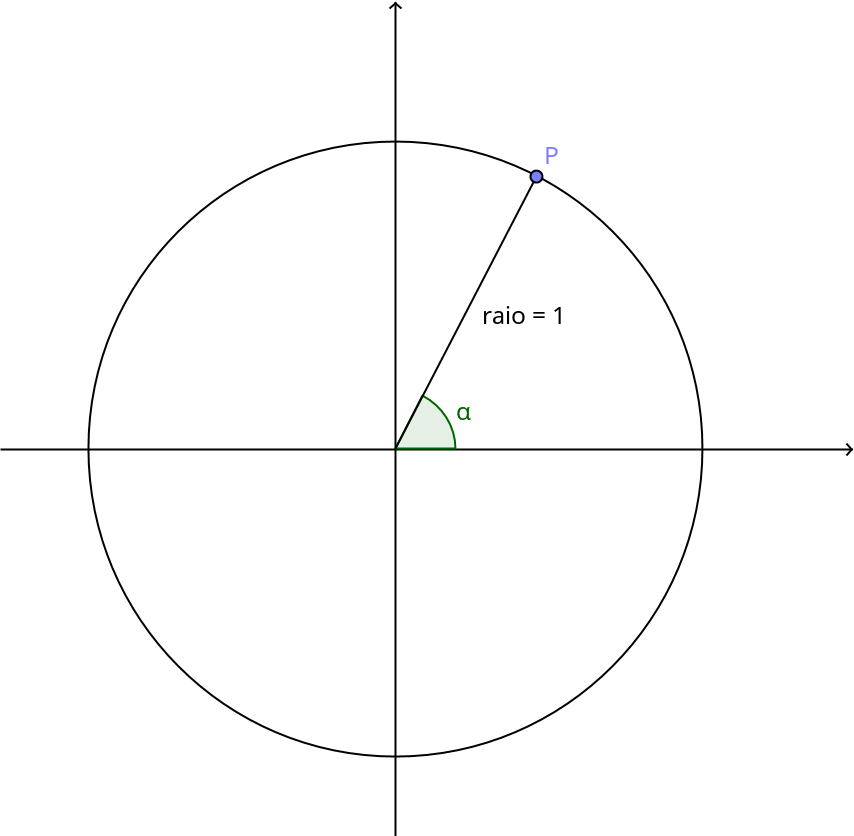
\includegraphics[width=0.5\textwidth]{./img/c6q15.png}
\end{figure}

\begin{questao}
Considerando a figura acima:
\begin{enumerate}[a)]
\item Como a coordenada $X$ do ponto $P$ pode ser obtido em termos do ângulo $\alpha$?
\item Como a coordenada $Y$ do ponto $P$ pode ser obtido em termos do ângulo $\alpha$?
\item Se considerarmos $\alpha$ como parâmetro, como ficaria a equação paramétrica da circunferência mostrada acima?
\end{enumerate} 
\end{questao}

A simplicidade dessa equação paramétrica é um dos motivos dela ser tão amplamente utilizada, tanto para descrever curvas mais complexas quanto para calcular integrais.

\subsection*{Explorado a forma paramétrica da circunferência}

Para finalizar esse capítulo, vamos explorar um pouco mais a forma paramétrica  da circunferência.

As questões a seguir são um pouco mais abertas do que as que você resolveu até agora e você vai precisar explorá-las um pouco mais autonomamente para conseguir resolvê-las. Por serem mais abertas, essas questões não possuem resposta no gabarito. Discuta as suas soluções com seus colegas e tutor.

\begin{questao}
Você obteve a equação $(x;y)=(\cos(t);\sin(t))$ para a circunferência de centro na origem e raio $1$ na questão anterior. Quais são as semelhanças e diferenças entre ela e a curva obtida pela equação $(x;y)=(\sint);\cos(t))$?
\end{questao}

\begin{questao}
Esboce a curva gerada pela equação paramétrica $(x;y)=(3\cos(t);4\sin(t))$. Como você descreveria essa curva?
\end{questao}

\begin{questao}
Qual deve ser a equação paramétrica da circunferência com centro na origem e raio igual a $3$?
\end{questao}

\begin{questao}
Qual deve ser a equação paramétrica da circunferência de raio $1$ e centro em $(2;3)$?
\end{questao}

\newpage

\section{Rumo ao livro-texto}

Neste capítulo, discutido diferentes formas de representar retas no plano cartesiano, ou seja, em um contexto com duas dimensões. Porém, em Geometria Analítica, você normalmente vai lidar com objetos no espaço, ou seja, em um contexto com três dimensões.

Essa mudança acrescenta um certo nível de dificuldade, mas quase tudo que discutidos aqui pode ser extrapolado ou usado como referência para entender o que ocorre em três dimensões. Por esse motivo, ao invés de resolver e propor uma questão do livro texto nesta seção, vamos sugerir uma leitura. Se você completou as questões propostas neste capítulo, sugerimos que você leia a seção 4.1 do livro \sugestao{Matrizes, Vetores e Geometria Analítica} na qual o autor introduz as equações de planos e retas no espaço. Preste atenção especial aos exemplos e não se preocupe com as demonstrações na sua primeira leitura (volte a elas no futuro).

Com isso, esperamos que você consiga dar mais significados aos conceitos que serão discutidos na disciplina.

\newpage

\section{Gabarito}

Confira as respostas para as questões e \textbf{não se esqueça de registrar o seu progresso}.

\noindent\textbf{Questão 1:} 

\begin{figure}[h]
\centering
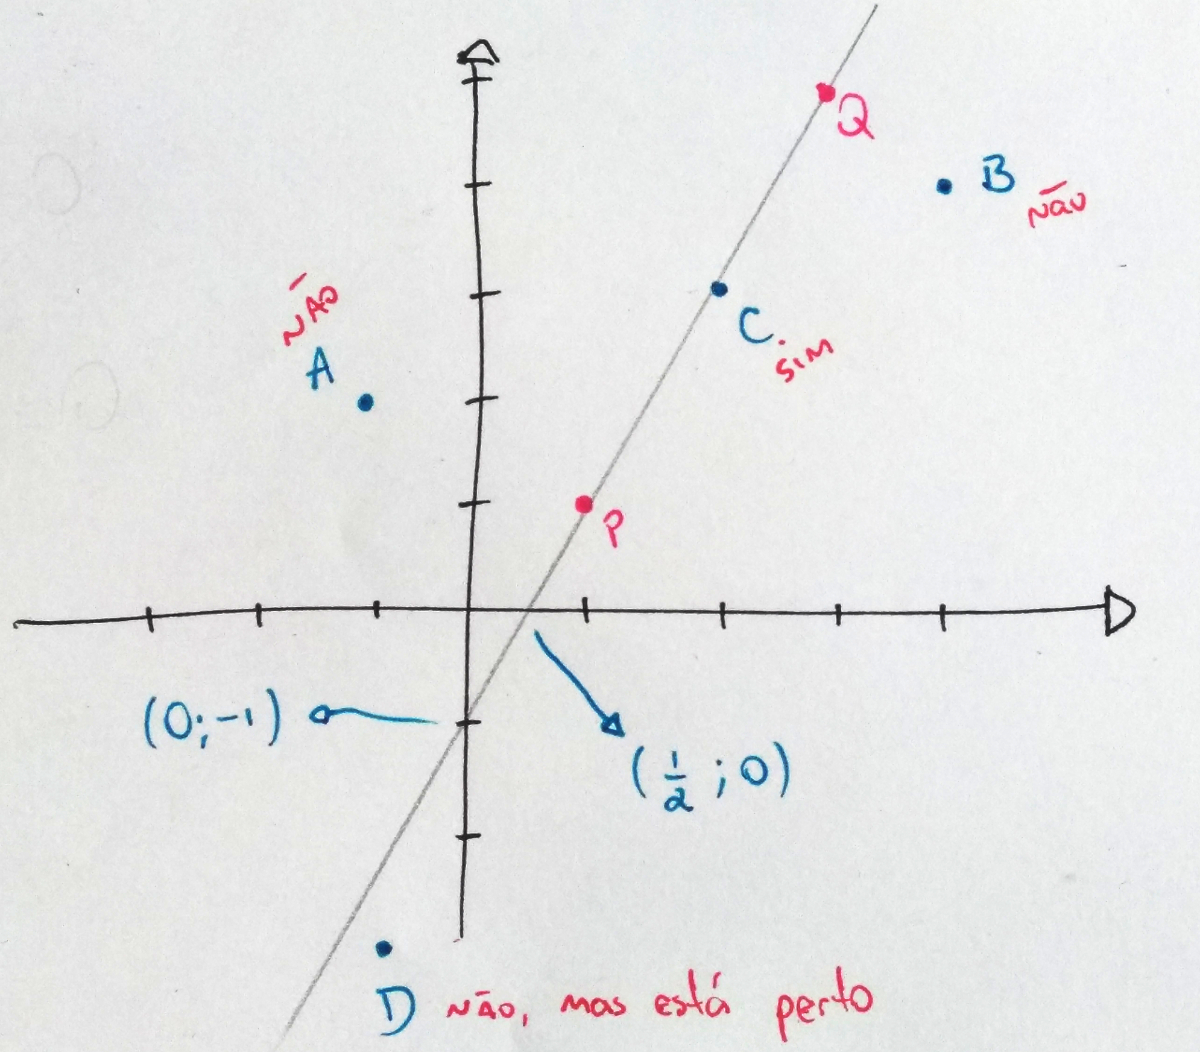
\includegraphics[width=0.5\textwidth]{./img/c6g1.jpg}
\end{figure}

\noindent\textbf{Questão 2:} a) $y=2x-1$.

\noindent\textbf{Questão 3:} a) $(10;19)$ e $(-1;-3)$, b) $(1/2;0)$ e $(0;-1)$, c) Apenas $C$ e $D$.

\noindent\textbf{Questão 4:} 

\begin{figure}[h]
\centering
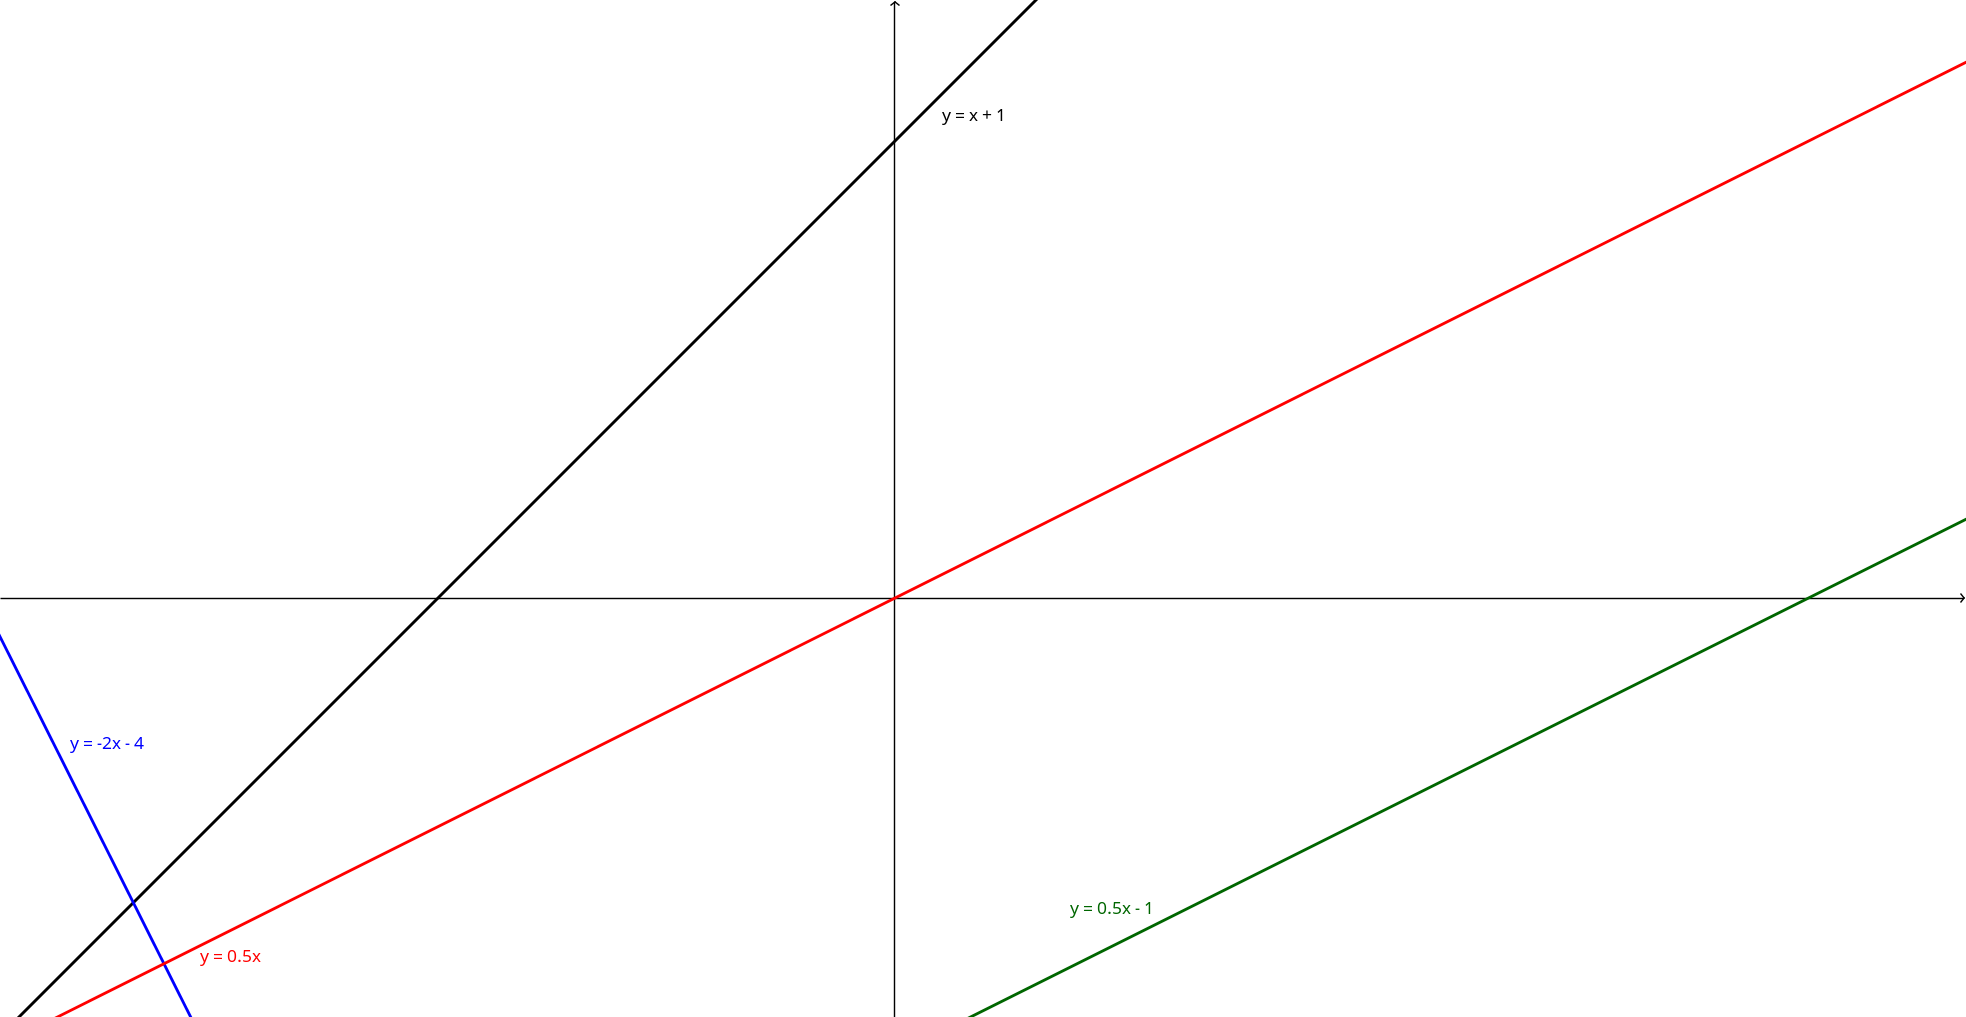
\includegraphics[width=0.5\textwidth]{./img/c6g4.png}
\end{figure}

\noindent\textbf{Questão 5:} $y=2x-2$, por exemplo.

\noindent\textbf{Questão 6:} a) $(2/3;0)$ e $(0;1)$, b) cheque com seu tutor ou colega.

\noindent\textbf{Questão 7:} 

\begin{figure}[h]
\centering
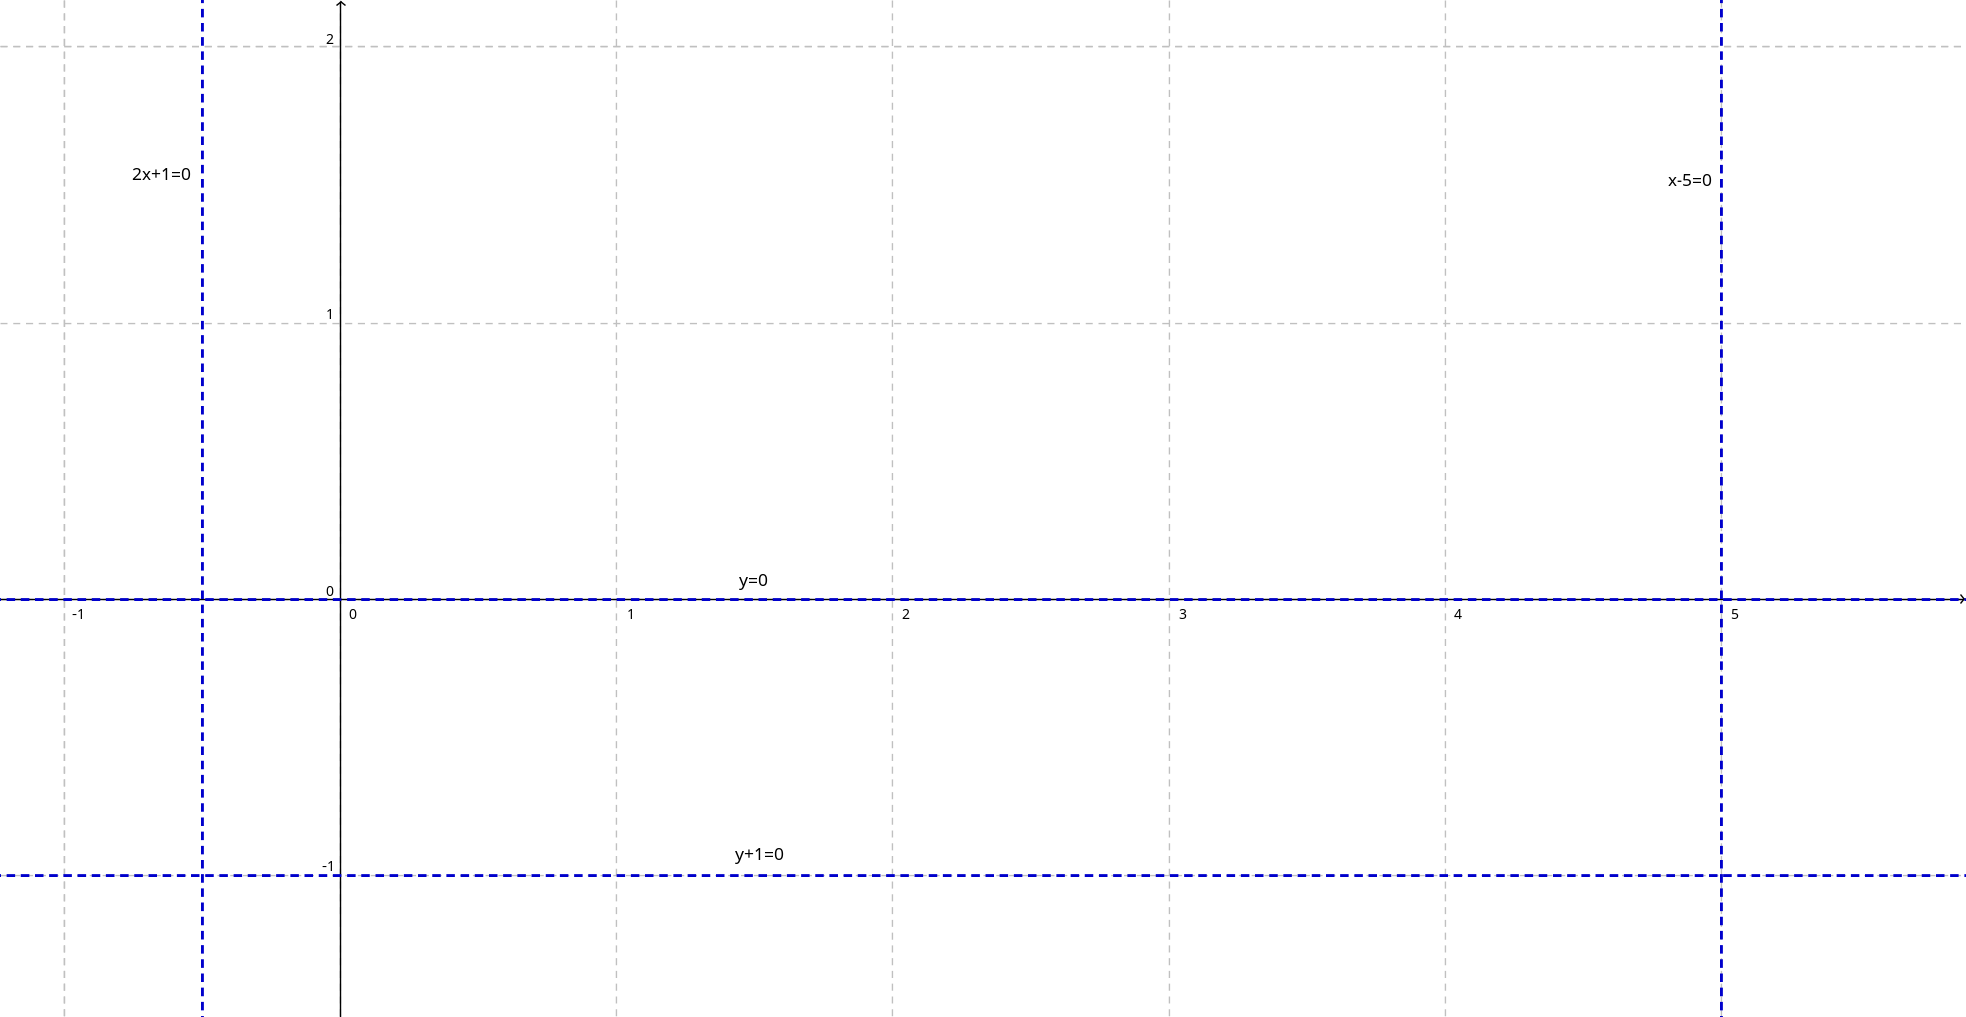
\includegraphics[width=0.5\textwidth]{./img/c6g7.png}
\end{figure}

\noindent\textbf{Questão 8:} b) $(-1;2)$ é uma possibilidade correta.

\noindent\textbf{Questão 9:} a) e b) abaixo, c)$2y+x-3=0$, d) $-y+5x-13=0$.

\begin{figure}[h]
\centering
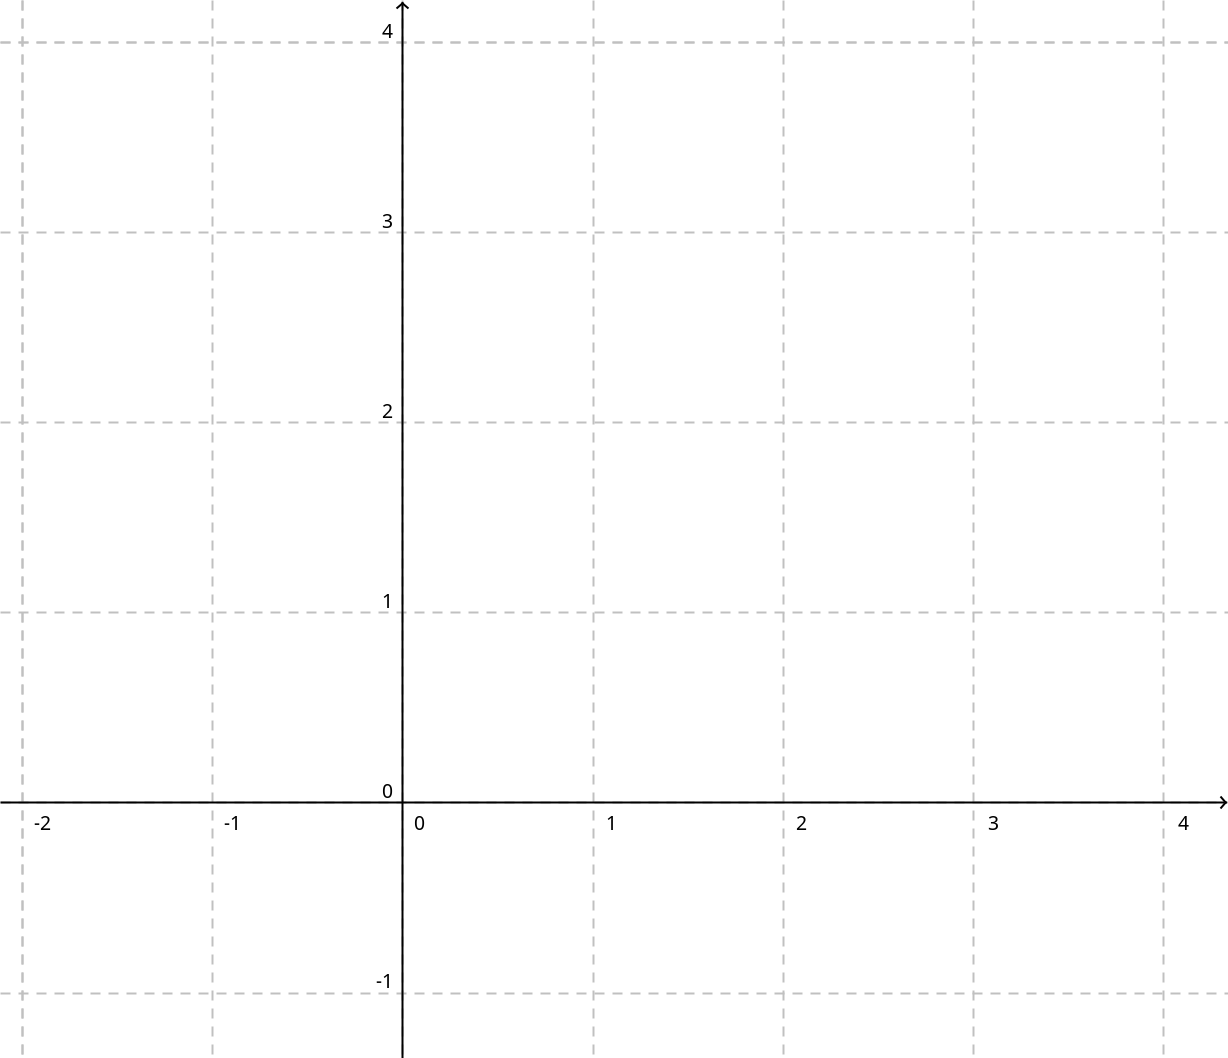
\includegraphics[width=0.7\textwidth]{./img/c6q9.png}
\end{figure}

\noindent\textbf{Questão 10:} a) $(-1;3)$, $(3;5)$ e $(-3;2)$, c) $t=-3$ e $t=1/2$.

\noindent\textbf{Questão 11:} b) $y=2x-1$, c) $y-2x+1=0$, d) $\overrightarrow{V}=(-2;1)$, e) $(x;y)=(1;1)+(2;4) \cdot t$.

\noindent\textbf{Questão 12:} a) $(x-2)^2+(y-1)^2=3^2$, b) $x^2+y^2=1$, c) $(1;-3)$ e $r=2$.

\noindent\textbf{Questão 13:} $(-1;+4)$ e $r=2$.

\noindent\textbf{Questão 15:} a) $x=\cos(\alpha)$, b) $y=\sin(\alpha)$,  c) $(x;y)=(\cos(\alpha);\sin(\alpha))$.

\newpage

\section{Registro de progresso}

Essa parte por enquanto fica com conteúdo vazio até que seja decidido como será feito o controle do progresso.
\vspace{5cm}

\section{Auto-avaliação final}
Avalie o quanto você acha que sabe sobre os seguintes itens após ter resolvido as questões deste capítulo.

\begin{center}
 \begin{tabular}{|p{35mm}||p{15mm}|p{15mm}|p{15mm}|p{15mm}|} 
 \hline
   & Nada & Muito pouco & Noções gerais & Bastante\\
 \hline
 Traçar o gráfico de uma reta dada a sua equação &  &  &  &  \\ 
 \hline
 Obter a equação de uma reta dados dois pontos &  &  &  &  \\
 \hline
 Identificar a equação de uma circunferência &  &  &  &  \\
 \hline
\end{tabular}
\end{center}

Cheque como foi o seu progresso comparando essas respostas com as que você deu antes de estudar este capítulo. Caso você não tenha atingido o nível ``Bastante''  em algum dos tópicos acima, liste abaixo qual ação concreta você fará nos próximos dias para atingi-lo:

\vspace{0.3cm}

\noindent\rule{\linewidth}{0.4pt}

\noindent\rule{\linewidth}{0.4pt}

\noindent\rule{\linewidth}{0.4pt}

\end{document}
